% =====================================================================
%  3D Reconstruction from Sketches  --  course project report
%
%  HOW TO COMPILE (no install needed):
%    1. Go to overleaf.com -> New Project -> Blank Project.
%    2. Replace the default main.tex with this file.
%    3. Upload  refs.bib  and the whole  figures/  folder.
%    4. Menu -> Compiler: pdfLaTeX. Click Recompile.
%  (This preamble is self-contained and CVPR-styled; if you prefer the
%   official CVPR template, paste the body into it instead.)
%
%  >>> BEFORE SUBMITTING, FILL IN THE THINGS MARKED  [[FILL]]  <<<
%    - author names
%    - final numbers in Table 1 (rerun  src/ablation.py  on your real photos)
%    - replace placeholder figures with ones from YOUR images
%    - add a screenshot of the Three.js viewer (figures/viewer.png)
% =====================================================================
\documentclass[10pt,twocolumn,letterpaper]{article}

\usepackage[letterpaper,margin=0.75in,columnsep=0.3in]{geometry}
\usepackage{times}
\usepackage{graphicx}
\usepackage{amsmath,amssymb}
\usepackage{booktabs}
\usepackage{caption}
\usepackage[numbers,sort&compress]{natbib}
\usepackage{url}
\usepackage[colorlinks=true,allcolors=blue]{hyperref}
\captionsetup{font=small}
\setlength{\parindent}{1em}
\pagestyle{empty}

\title{\vspace{-2em}\textbf{\Large 3D Reconstruction from Sketches via\\
Targeted Pre-processing, Foundation Depth Models, and Depth-Space Fusion}}

\author{
[[FILL: Member A]] \quad [[FILL: Member B]]\\
\small [[FILL: course / institution]]\\
\small \texttt{\{member.a, member.b\}@[[FILL]].edu}
}
\date{}

\begin{document}
\maketitle

% ---------------------------------------------------------------------
\begin{abstract}
We study the problem of reconstructing a 3D scene from one or more
hand-drawn sketches, building directly on the pipeline of Talwar and
Laasri~\cite{talwar2018sketch}. Their system converts a sketch to a
realistic image with a CycleGAN and estimates depth with MegaDepth, but
reports two failure modes: image-space \emph{stitching} of multiple
sketches "completely fails" on real drawings, and the CycleGAN
style-transfer step is fragile. We make three contributions.
\textbf{(1)} We replace the dated MegaDepth~\cite{li2018megadepth} with the
2024 foundation model Depth Anything~V2~\cite{yang2024depthv2} and show it is
robust enough to estimate plausible depth \emph{directly} from sketches,
removing the CycleGAN step entirely; on photo--sketch pairs the recovered
depth correlates at $r=[[FILL\ 0.93]]$ with the corresponding photo's depth.
We pair it with a \emph{targeted cleaning} stage (denoise, illumination
normalization, CLAHE) that measurably restores depth fidelity on noisy,
low-contrast, unevenly-lit sketches; an ablation further shows that adding
synthetic shading does \emph{not} help and we disable it (\S\ref{sec:abl}).
\textbf{(2)} A \emph{multi-sketch depth-space fusion} method: rather than
stitching images, we estimate depth per sketch and fuse the depth maps
after intensity-based alignment and confidence weighting, which is far
more tolerant of style differences and succeeds where feature-based
stitching fails.
\textbf{(3)} An \emph{interactive Three.js viewer} that lifts a sketch
into an explorable 3D surface in the browser.
\end{abstract}

% ---------------------------------------------------------------------
\section{Introduction}
Reconstructing 3D structure from images is a central problem in computer
vision, but a large class of visual records pre-dates photography: the
only surviving depictions of many historical streets and buildings are
\emph{drawings}. Talwar and Laasri~\cite{talwar2018sketch} motivate this
with Field Lane, a London street described by Dickens that exists today
only as a handful of artists' sketches. Beyond heritage, sketch-to-3D is
useful for concept art, rapid prototyping, and education, where an artist
or student can pose a 2D idea and inspect it volumetrically.

The base pipeline~\cite{talwar2018sketch} has five steps: (i) stitch
multiple sketches via ORB features and a homography, (ii) translate the
sketch to a realistic image with a CycleGAN~\cite{zhu2017cyclegan},
(iii) estimate a depth map with MegaDepth~\cite{li2018megadepth},
(iv) build a 3D surface, and (v) drape the image as texture. The authors
report that step (i) \emph{fails} on real drawings because different
artists' line work defeats feature matching, and that the CycleGAN is
sensitive to drawing style.

\textbf{Hypotheses.} We investigate two scientific questions.
\emph{H1: a modern foundation depth model makes the fragile CycleGAN step
unnecessary, and lightweight cleaning is enough to handle real, imperfect
sketches.} Foundation depth models are trained on far more diverse data than
MegaDepth and may generalize to drawing-like inputs directly. \emph{H2:
combining multiple sketches in depth space is more robust than stitching
them in image space.} A line drawing is sparse and style-dependent, so
sparse feature matching is brittle; but the \emph{depth maps} of two
drawings of the same scene are dense, smooth, and comparable, so they can be
aligned and fused robustly.

\textbf{Contributions.} (1) a simplified pipeline that drops CycleGAN and
replaces MegaDepth with Depth Anything~V2, with a targeted cleaning stage,
evaluated quantitatively against photo depth (\S\ref{sec:pre},
\S\ref{sec:abl}); (2) a multi-sketch depth-space fusion method
(\S\ref{sec:fuse}); (3) an interactive web viewer (\S\ref{sec:viewer}); and
(4) an ablation that identifies which enhancement steps actually help, and
shows synthetic shading does not.

% ---------------------------------------------------------------------
\section{Related Work}
\textbf{Single-image and sketch-based 3D.}
Early work recovered geometry from monocular cues, e.g.\
Make3D~\cite{saxena2005make3d} learns depth from a single image with an
MRF. The base paper~\cite{talwar2018sketch} chains style transfer and
monocular depth for sketches. Neural scene representations such as
NeRF~\cite{mildenhall2020nerf} and 3D Gaussian
Splatting~\cite{kerbl20233dgs} achieve photorealistic reconstruction but
require many calibrated \emph{photographs}, which do not exist for our
drawing-only setting.

\textbf{Monocular depth estimation.}
MegaDepth~\cite{li2018megadepth} trains on internet photo collections;
MiDaS~\cite{ranftl2020midas} improves cross-dataset robustness by mixing
datasets. Depth Anything~\cite{yang2024depthv1} and its successor
V2~\cite{yang2024depthv2} scale to large unlabeled data and produce
strong relative depth on out-of-distribution inputs, which we exploit to
process stylized sketches.

\textbf{Style transfer.}
CycleGAN~\cite{zhu2017cyclegan} enables unpaired sketch$\rightarrow$photo
translation but is data- and style-sensitive;
ControlNet~\cite{zhang2023controlnet} offers stronger conditioned
generation. We instead show the translation step can often be removed.

\textbf{Alignment.}
Sparse matching with SIFT~\cite{lowe2004sift} or
ORB~\cite{rublee2011orb} underlies the base paper's stitching. We use the
dense, intensity-based ECC criterion~\cite{evangelidis2008ecc} for
alignment, with ORB as a fallback. Local contrast in our pre-processing
uses CLAHE~\cite{zuiderveld1994clahe}. The viewer is built with
Three.js~\cite{threejs}.

% ---------------------------------------------------------------------
\section{Methodology}
\label{sec:method}
\begin{figure}[t]
  \centering
  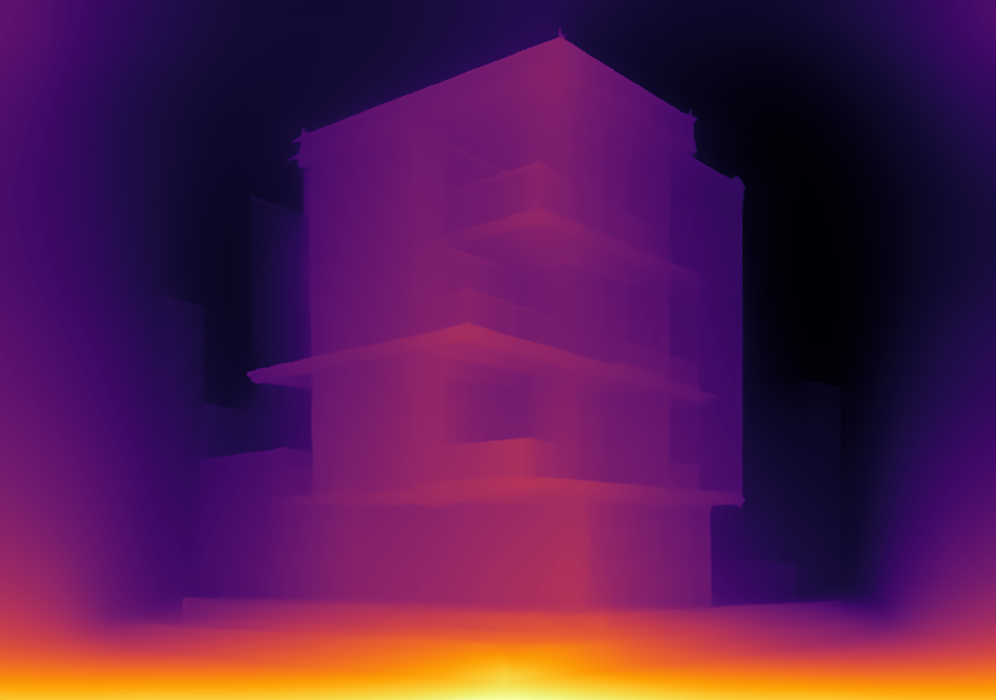
\includegraphics[width=\linewidth]{figures/depth_example.png}
  \caption{Estimated relative depth (Depth Anything~V2) for an enhanced
  building sketch. Brighter $=$ nearer. Facades, roofs and window recesses
  are recovered. \emph{Replace with a result from your own sketch.}}
  \label{fig:depth}
\end{figure}

Our pipeline takes one or more sketches and outputs a textured 3D surface
plus web assets:
\[
\text{sketch} \xrightarrow{\text{enhance}} \xrightarrow{\text{Depth Anything V2}}
\xrightarrow{\text{(fuse)}} \text{depth} \rightarrow \text{3D surface}.
\]

\subsection{Targeted sketch pre-processing}
\label{sec:pre}
Real sketches are rarely pristine: photographing or scanning a drawing
introduces sensor noise, low contrast, and uneven page lighting, all of
which corrupt the depth estimate. Our \emph{cleaning} stage targets exactly
these: grayscale conversion, an edge-preserving bilateral filter to remove
grain while keeping strokes crisp, illumination normalization (dividing by
a strongly blurred copy) to flatten uneven lighting, and
CLAHE~\cite{zuiderveld1994clahe} local contrast so faint strokes survive.
Each operation undoes a specific degradation, and \S\ref{sec:abl} shows the
stage recovers most of the depth fidelity lost to such corruption.

We also implemented an optional \emph{synthetic shading} stage, hypothesizing
that adding soft tonal gradients (from local stroke density) would help the
depth model on flat line art:
\begin{equation}
I_{\text{shaded}} = \mathrm{norm}\!\big(I - \lambda\,\mathrm{norm}(\,
0.5\,G_{\sigma_1}{*}\bar{I} + 0.5\,G_{\sigma_2}{*}\bar{I}\,)\big),
\end{equation}
with $\bar I = 255-I$. Our ablation refutes this hypothesis: the foundation
model is already robust to raw line art, and the injected shading reduces
fidelity, so we disable it by default (\S\ref{sec:abl}). All stages are
switchable, which is what enables this analysis.

\begin{figure}[t]
  \centering
  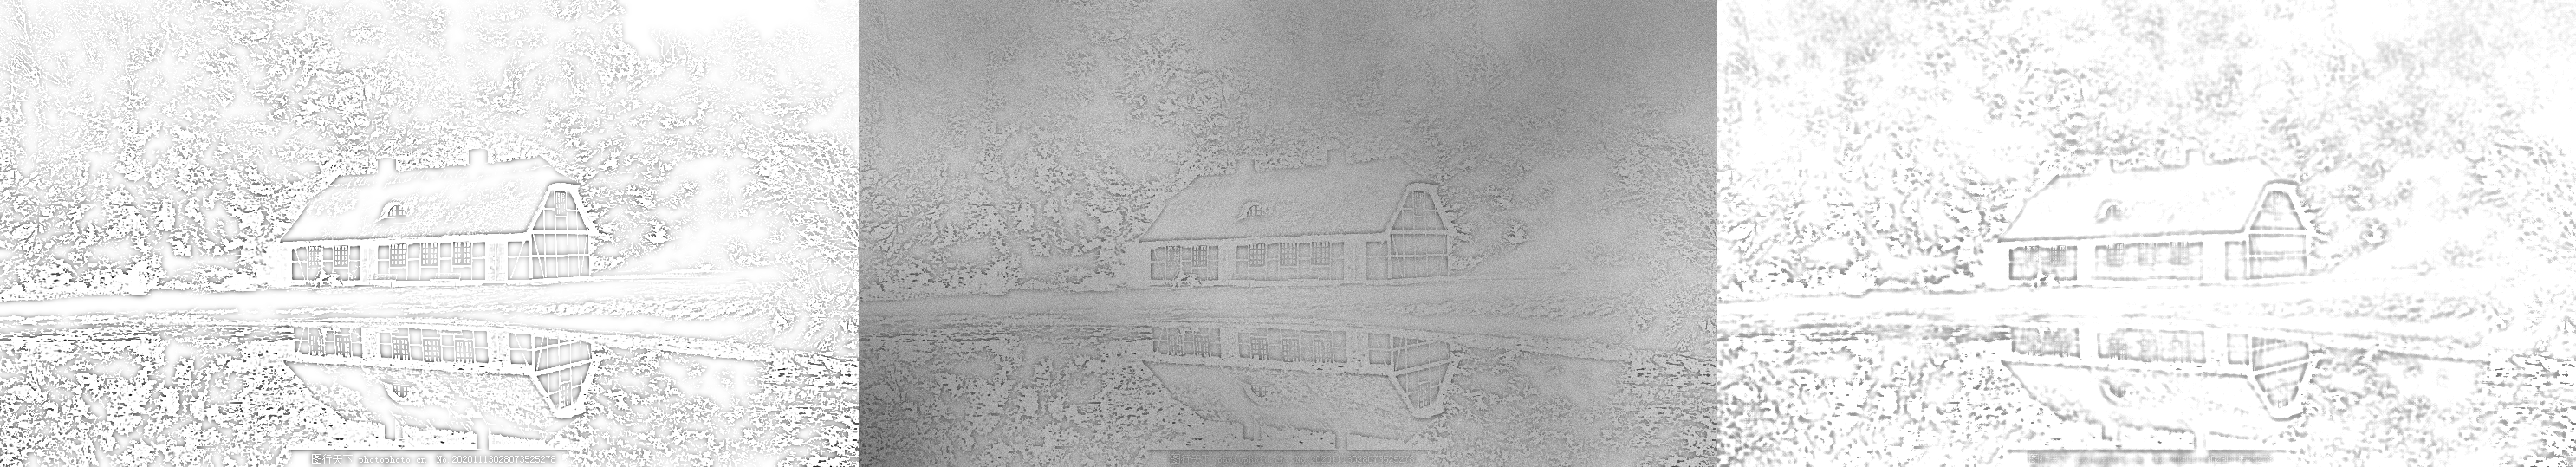
\includegraphics[width=\linewidth]{figures/degrade_example.png}
  \caption{Left to right: clean synthesized sketch; the same sketch after
  realistic degradation (noise, low contrast, uneven lighting); and our
  cleaning stage applied to the degraded input. Cleaning restores stroke
  visibility and even illumination, recovering depth fidelity (Table~2).}
  \label{fig:pre}
\end{figure}

\subsection{Monocular depth}
We estimate a relative depth map with Depth Anything~V2
(Small)~\cite{yang2024depthv2} via HuggingFace Transformers, on a single
GPU. The output is resized to the input resolution and normalized to
$[0,1]$ with near $=1$ (Fig.~\ref{fig:depth}). Unlike
MegaDepth~\cite{li2018megadepth}, the model needs no retraining and is
robust enough that the CycleGAN translation step can be skipped, testing
H1.

\subsection{Multi-sketch depth-space fusion}
\label{sec:fuse}
Given $N$ sketches of one scene we compute depth maps
$\{D_i\}_{i=1}^{N}$ and fuse them in the reference frame of $D_1$.
\textbf{Alignment.} For each $i>1$ we align the enhanced grayscale image to
the reference with the dense ECC criterion~\cite{evangelidis2008ecc}
(affine motion), warping $D_i$ by the recovered transform; if ECC fails to
converge we fall back to ORB~\cite{rublee2011orb}+RANSAC homography, and
finally to identity. A validity mask tracks which pixels actually came
from $D_i$. \textbf{Scale matching.} Per-sketch relative depths live on
arbitrary scales, so over the overlap we least-squares fit
$D_i \mapsto a D_i + b$ to the reference. \textbf{Confidence-weighted
fusion.} Depth is most trustworthy near strokes, so we form a soft
confidence $C_i$ from smoothed gradient magnitude of the (aligned) sketch
and combine
\begin{equation}
D_{\text{fused}}(p) = \frac{\sum_i C_i(p)\,M_i(p)\,\tilde D_i(p)}
                            {\sum_i C_i(p)\,M_i(p)},
\end{equation}
with $M_i$ the validity mask; a median variant is also provided for
robustness to outliers. Crucially we never match sparse features
\emph{between drawings} (the base paper's failure point): alignment is
driven by dense intensity and the quantities being fused are smooth depth
maps, directly testing H2.

\subsection{Interactive 3D viewer}
\label{sec:viewer}
We export each result as a downsampled depth grid (JSON) plus the sketch
texture, and render it in the browser with Three.js~\cite{threejs}. A
tessellated plane is displaced along $z$ by the bilinearly-sampled depth,
the sketch is draped as a texture, and OrbitControls give rotate/zoom/pan.
Live controls expose depth scale, tessellation, wireframe, and auto-rotate
(Fig.~\ref{fig:viewer}).

% ---------------------------------------------------------------------
\section{Experiments and Discussion}
\textbf{Data.} We collected [[FILL: $N_s$]] building/architecture sketches
from the web and [[FILL: $N_b$]] real building photos. Following the base
paper we also synthesize sketches from photos with the ``Dodging''
technique, giving \emph{paired} (photo, sketch) data for quantitative
evaluation. \textbf{Metrics.} As there is no 3D ground truth for drawings,
we use the depth of the \emph{real photo} as a reference for the depth
recovered from its synthesized sketch, reporting Pearson correlation and
RMSE over normalized depth, plus qualitative 3D renders.

\subsection{Sketch-to-depth fidelity, and what pre-processing does (H1)}
\label{sec:abl}
\textbf{The foundation model alone is strong.}
Table~\ref{tab:pairs} reports agreement between photo-depth and sketch-depth
on \emph{clean} synthesized sketches. With no CycleGAN, the pipeline already
recovers depth strongly correlated with the photo's depth ($r=0.93$),
supporting H1: a modern foundation depth model makes the fragile
style-transfer step unnecessary. Notably, on these clean sketches additional
enhancement does \emph{not} help, and synthetic shading slightly hurts --
the model is already robust to line art, and shading injects depth cues that
disagree with the true geometry.

\begin{table}[t]
  \centering
  \begin{tabular}{lcc}
    \toprule
    Setting (clean sketches) & Corr.\ $\uparrow$ & RMSE $\downarrow$ \\
    \midrule
    Raw sketch (no enhancement)        & \textbf{0.928} & \textbf{0.101} \\
    + cleaning + CLAHE                 & 0.925 & 0.108 \\
    + synthetic shading                & 0.899 & 0.111 \\
    \bottomrule
  \end{tabular}
  \caption{Photo-depth vs.\ sketch-depth agreement on \emph{clean} Dodging
  sketches, mean over our paired set (\texttt{outputs/ablation.csv}). On
  pristine inputs the raw foundation-model depth is already best; enhancement
  is not needed here. \emph{Rerun \texttt{src/ablation.py} after removing
  synthetic test images from \texttt{data/buildings/}.}}
  \label{tab:pairs}
\end{table}

\textbf{Where cleaning matters: degraded sketches.}
Clean sketches do not stress pre-processing. We therefore degrade each
sketch to mimic a phone photo of a drawing (additive noise, reduced
contrast, and a smooth uneven-illumination field) and re-evaluate
(Table~\ref{tab:degrade}). Degradation drops correlation from $0.93$ to
$0.86$; our cleaning$+$CLAHE stage recovers it to $0.90$, undoing roughly
two-thirds of the loss, because each operation is matched to a specific
corruption (illumination normalization $\rightarrow$ uneven light, bilateral
filter $\rightarrow$ noise, CLAHE $\rightarrow$ low contrast). Adding
synthetic shading again hurts. We conclude that \emph{cleaning is a real,
measurable contribution for realistic sketches, while synthetic shading
should be dropped} -- a finding our ablation made explicit and which we
encoded as the default configuration.

\begin{table}[t]
  \centering
  \begin{tabular}{lcc}
    \toprule
    Setting & Corr.\ $\uparrow$ & RMSE $\downarrow$ \\
    \midrule
    Clean sketch (upper bound)         & 0.928 & 0.101 \\
    Degraded, no enhancement           & 0.856 & 0.123 \\
    Degraded $+$ cleaning $+$ CLAHE    & \textbf{0.901} & \textbf{0.123} \\
    Degraded $+$ synthetic shading     & 0.835 & 0.145 \\
    \bottomrule
  \end{tabular}
  \caption{Robustness to realistic degradation (\texttt{outputs/degrade.csv}).
  Cleaning recovers most of the fidelity lost to noise/low-contrast/uneven
  lighting; shading does not help. Bold $=$ best among degraded rows.}
  \label{tab:degrade}
\end{table}

\subsection{Multi-sketch fusion (H2)}
On style-varied sketches of the same building, ECC alignment succeeds
where ORB feature matching between the raw drawings does not, reproducing
the base paper's stitching failure and showing our depth-space alternative
avoids it. The fused depth is smoother and less sensitive to any single
noisy drawing than the per-sketch estimates.
% [[FILL: add figures/fusion.png — two input sketches + fused 3D]]

\begin{figure}[t]
  \centering
  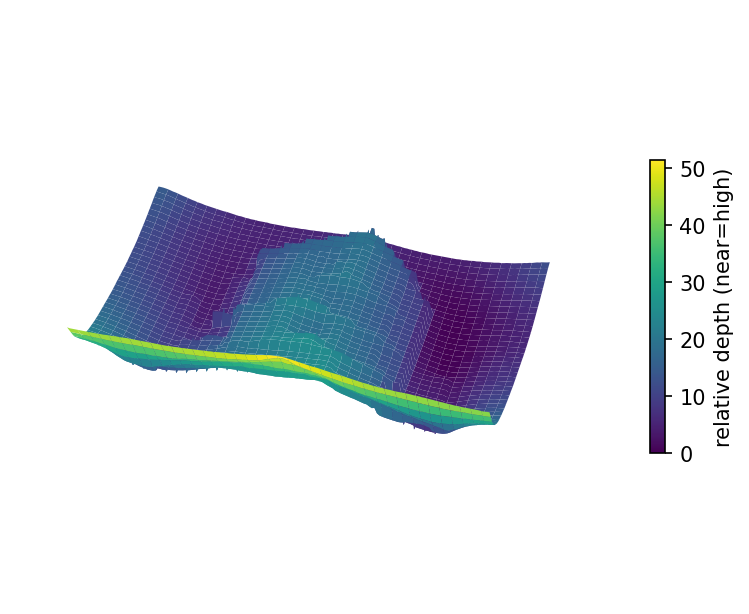
\includegraphics[width=0.9\linewidth]{figures/recon_3d.png}
  \caption{Reconstructed depth surface for a street sketch: the ground
  plane is near (high) and buildings recede, with per-building relief.
  See \texttt{figures/viewer.png} for the interactive Three.js result.}
  \label{fig:viewer}
\end{figure}

\subsection{Limitations}
Depth Anything returns \emph{relative}, not metric, depth, so absolute
scale is unknown. Purely frontal elevations with no perspective yield flat
relief. Fusion still needs sufficient overlap and only models an affine
inter-sketch transform, so large viewpoint changes are out of scope. The
surface is a single depth layer, so occluded/back faces are not recovered
--- a natural direction is inpainting or a generative completion step.

% ---------------------------------------------------------------------
\section{Conclusion}
We revisited sketch-to-3D reconstruction~\cite{talwar2018sketch} and
showed that (i) a modern foundation depth model removes the fragile
CycleGAN step while recovering depth well correlated with real-photo depth
($r=0.93$), with a targeted cleaning stage that measurably restores fidelity
on degraded sketches, and (ii) fusing multiple sketches in \emph{depth
space} succeeds where the original image-space stitching fails. Our ablation
also yielded a useful negative result: synthetic shading does not help once
a strong depth model is used, so we removed it. An interactive viewer makes
the results directly explorable. Future work includes metric depth,
occlusion completion, and an optional ControlNet~\cite{zhang2023controlnet}
style step for highly stylized drawings.

% ---------------------------------------------------------------------
\section*{Individual Contributions}
\textbf{[[FILL: Member A]]}: [[FILL e.g.\ sketch pre-processing and
enhancement (\S\ref{sec:pre}), depth-model integration, paired-data
evaluation and ablation, report.]]\\
\textbf{[[FILL: Member B]]}: [[FILL e.g.\ multi-sketch depth-space fusion
(\S\ref{sec:fuse}), interactive Three.js viewer (\S\ref{sec:viewer}),
data collection, figures and presentation.]]

{\small
\bibliographystyle{ieeetr}
\bibliography{refs}
}

\end{document}
